%----------------------------------------------------------------------------------------
%	PACKAGES AND OTHER DOCUMENT CONFIGURATIONS
%----------------------------------------------------------------------------------------

\documentclass[twoside,fontsize=12pt]{article}
%\documentclass[oneside]{article}
\usepackage{lipsum} % Package to generate dummy text throughout this template
\usepackage{graphicx}

%\usepackage[sc]{mathpazo} % Use the Palatino font
\usepackage[T1]{fontenc} % Use 8-bit encoding that has 256 glyphs
\linespread{1.5} % Line spacing - Palatino needs more space between lines
\usepackage{microtype} % Slightly tweak font spacing for aesthetics
\usepackage{listings}
\usepackage[hmarginratio=1:1,top=32mm,columnsep=20pt]{geometry} % Document margins
%\usepackage{multicol} % Used for the two-column layout of the document
\usepackage[hang, small,labelfont=bf,up,textfont=it,up]{caption} % Custom captions under/above floats in tables or figures
\usepackage{booktabs} % Horizontal rules in tables
\usepackage{float} % Required for tables and figures in the multi-column environment - they need to be placed in specific locations with the [H] (e.g. \begin{table}[H])
\usepackage[hidelinks]{hyperref} % For hyperlinks in the PDF

\usepackage{lettrine} % The lettrine is the first enlarged letter at the beginning of the text
\usepackage{paralist} % Used for the compactitem environment which makes bullet points with less space between them
\usepackage{chngcntr}
\counterwithout{figure}{section}
\usepackage{abstract} % Allows abstract customization
\renewcommand{\abstractname}{}    % clear the title
\renewcommand{\absnamepos}{empty}
\renewcommand{\abstractnamefont}{\normalfont\bfseries} % Set the "Abstract" text to bold
\renewcommand{\abstracttextfont}{\normalfont\small\itshape} % Set the abstract itself to small italic text
\usepackage[super, sort&compress]{natbib}
\setlength{\bibsep}{0.0pt}
\bibliographystyle{unsrtnat}
\usepackage{titlesec} % Allows customization of titles
\renewcommand\thesection{\Roman{section}} % Roman numerals for the sections
\renewcommand\thesubsection{\Roman{subsection}} % Roman numerals for subsections
\titleformat*{\section}{\LARGE\scshape\centering}
\renewcommand{\bibsection}{\section*{\refname}}
\titleformat{\section}[block]{\LARGE\scshape\centering}{\thesection}{1em}{} % Change the look of the section titles
\titleformat{\subsection}[block]{\large\bfseries}{\thesubsection}{1em}{} % Change the look of the section titles
\titleformat{\subsubsection}[block]{\bfseries\textit}{\thesubsubsection}{0.1mm}{} % Change the look of the section titles
\usepackage[table,xcdraw]{xcolor}
\usepackage{caption}


\usepackage{fancyhdr} % Headers and footers
\pagestyle{fancy} % All pages have headers and footers
\fancyhead{} % Blank out the default header
\fancyfoot{} % Blank out the default footer
\fancyhf{}
\renewcommand{\headrulewidth}{0pt}
%\fancyhead[C]{Running title $\bullet$ November 2012 $\bullet$ Vol. XXI, No. 1} % Custom header text
\fancyfoot[RO,LE]{\thepage} % Custom footer text

%----------------------------------------------------------------------------------------
%	TITLE SECTION
%----------------------------------------------------------------------------------------

\title{\vspace{-15mm}\fontsize{18pt}{10pt}\normalfont\textbf{Exploring multi-level effects of structural variations in non-coding genomic regions in cancer\\ \vspace{4 mm} {{\footnotesize \textit{Linking and visualising data for dynamic  multidimensional biological data interpretation.}}}}} % Article title

\author{
\large
\textsc {RHWE (Robin) van der Weide}\thanks{Supervisor: Joep de Ligt, PhD}\\[2mm] 
\normalsize  BSc. Biology
\normalsize  MSc. Cancer Stem cells \& Developmental biology (honours program)
\normalsize  Utrecht Graduate School of Life Sciences 
%\normalsize \href{mailto:john@smith.com}{john@smith.com} % Your email address
\vspace{-5mm}
}
\date{}

%----------------------------------------------------------------------------------------

\begin{document}

\maketitle % Insert title

\thispagestyle{fancy} % All pages have headers and footers

%\vspace{3cm}
%\begin{figure}[H]
%    \centering
%    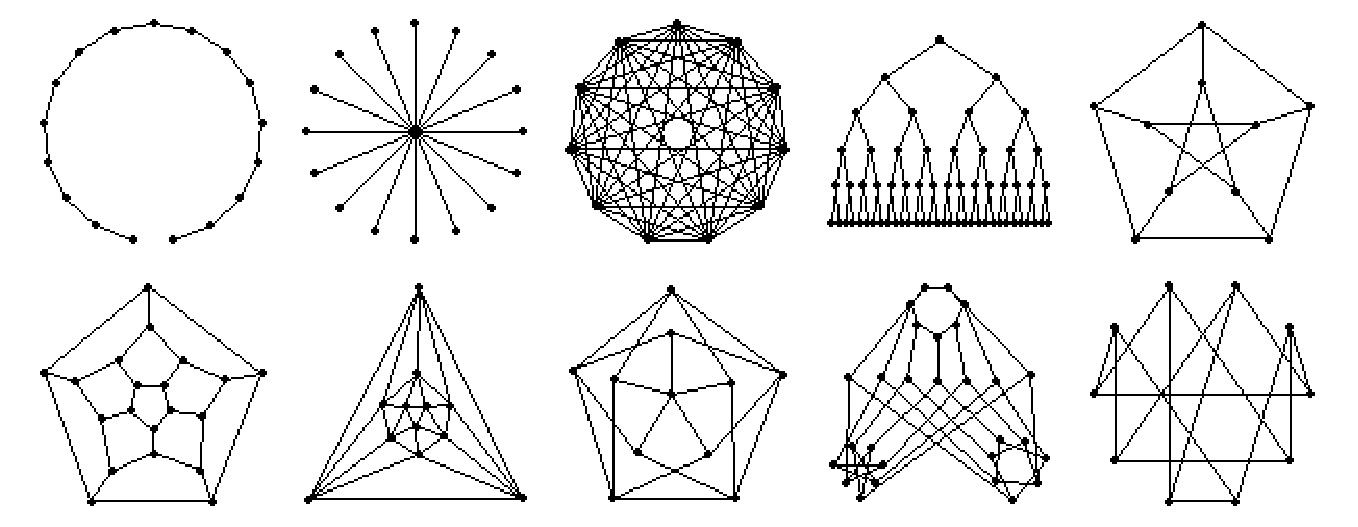
\includegraphics[width=1\textwidth]{graphs}
%   \end{figure}
%----------------------------------------------------------------------------------------
%	ABSTRACT
%----------------------------------------------------------------------------------------

\newpage
\renewcommand{\abstractname}{\begin{center}
Summary of the research
\end{center}}    % clear the title

\begin{abstract}
\noindent
To date, studies on non-coding regions of the genome, specifically in cancer, have been limited. This is mainly due to the complex nature of putative functional elements in these regions. Increased knowledge of these regions, through efforts such as the ENCODE-project, enabled researchers to initiate studies on the causality of non-coding variations in cancer\cite{Benko2009,Kurth2009}. 
The ongoing cost reduction of various omics-approaches coupled to high throughput research, has led an explosion of available data. However, the complexity of integrating and analysing these large datasets increases with every added omics-layer or dimension (e.g. time-series, treatments). When studying the effects of genetic variants in cancer, this complexity is further increased due to cancer-specific (e.g. heterogeneous samples, rapid evolution). The elucidation of structural variants is further complicated by the diversity in types and consequences of these genetic alterations.
\medskip

\noindent
The current methods for integrating and analysing multiple layers or dimensions have two major limitations in their design: scalability and generality (i.e. the possibility to easily add more levels or dimensions). Moreover, the sheer amount of data points makes it impossible to overview a dataset without filtering, dividing or restructuring the data. Integration of complex datasets is needed to better understand the complex biology of cancer\cite{Munoz2011}, but is greatly restricted by these limitations.
\medskip

\noindent Enter the Semantic Web and its Resource Description Framework (RDF). A simple and flexible framework for describing anything about anything.
% An example of such a RDF-instance (a triple) is "BRAF1 has the molecular function of binding calcium ion", which has these three parts: a subject (BRAF1), a predicate (molecular function) and an object (binding calcium ion). Another triple can then say something about the phosphorylated protein levels of this gene in a sample. Connecting these two triples would enable a researcher to find a possible pattern in the data (i.e. a gene, responsible for calcium ion binding, has a low phosphorylation level in the investigated sample). 
Since every type of data can be translated to this universal language, integration of large datasets of different levels and dimensions becomes possible and more feasable. When researchers  convert their local data to RDF, they can easily connect and combine it with public repositories,  making analyses more powerful. By using the SPARQL Protocol and RDF Query Language (SPARQL), retrieving and manipulating data in RDF is easily readable by both humans and computers. Researchers can subsequently visualise the SPARQL-results as a whole or filter them further.
\medskip

\noindent Here, we propose the use of semantic web technologies and visual analytics to decrease the complexity of integrating and visualizing multi-level and -dimensional biological data. These methods will enable further elucidation of the complex biology of, for example, cancer. Firstly, we will create the framework needed to design the missing tools for converting the most-used omics formats to RDF. Next, visualisations (based on visual analytics) of the biological RDF-data will be created, which will be used to perform previously impossible integration-focussed analyses on the consequences of structural variation in the non-coding regions of cancer-genomes.
\end{abstract}
\medskip

%%%%%%%%%%%%%%%%%%%%%%%%%%%%%%%
%	not needed for BIF
%%%%%%%%%%%%%%%%%%%%%%%%%%%%%%%


%\renewcommand{\abstractname}{\begin{center}
%Layman's summary
%\end{center}}    % clear the title

%\begin{abstract}\noindent
%The biomedical research community wants to be able to combine and analyse a multitude of biological signals in one experiment because the biology of, for example, cancer is so complex. However, integrating diverse sets of biological signals is currently a serious challenge. To overcome this, we propose the use of Semantic Web-methods: these are specially designed for integrating vast amounts of different data. Furthermore, it allows users to describe, analyse and test their data interactively and dynamically via visual representations displayed in the browser. These methods would enable researchers in- and outside of bioinformatics to more efficiently analyse and integrate datasets, making it easier to propose (and answer) research questions.

%A preliminary study shows the added value of such methods in biology: enabling researchers to describe, analyse and test 20 times more biological questions in the same time, compared to conventional methods. We propose to develop these methods further for the research-community (and biology in particular), enabling us to more effectively and systematically perform research on variations in the non-coding genomic regions in cancer. \\
%\medskip


%\end{abstract}

\noindent \textbf{Keywords:} structural variation, multi-level data integration, next-generation sequencing, cancer, visual analytics

%----------------------------------------------------------------------------------------
%	ARTICLE CONTENTS
%----------------------------------------------------------------------------------------
\newpage
\section*{Background, aims and approach}
\subsection*{Overall aim}
The aim of this project is to integrate and visualise multiple levels and dimensions of omics-data with methods of the Semantic Web. Moreover, these methods will be used to study the inter-level (e.g. transcriptome, proteome) consequences of structural variation in non-coding regions of the genome. Thus, this proposal has three sub-projects, which rely heavily on each other:

\begin{enumerate}
\item \textbf{Data-integration} 
Integration of Next Generation Sequencing(NGS) based data by using Semantic Web-methodologies to improve integrative bioinformatics in general and NGS-based multi-level and -dimensional research in particular.
\item \textbf{Visual analytics} 
Linking the Semantic-Web data to D3.js, enabling dynamic and interactive visualisation of RDF-data.
\item \textbf{Multi-level analysis} 
Multi-level and -dimensional integrative bioinformatics analysis to elucidate the consequences of genomic structural variations in non-coding regions in cancer.
\end{enumerate}

\subsection*{Scientific relevance and challenges} 
Finding causal genetic variation in the protein-coding regions of the genome has been the focus in the majority of genomics studies. However, these regions amount only to approximately two percent\cite{Lander2001}. One of the primary reasons behind this is the relative uncomplicated nature of studying coding regions, as consequences on lower levels (e.g. transcription, proteins) are traceable\cite{McLaren2010}. This is in contrast to the non-coding regions, which often do not show a linear effect on other levels\cite{Bird2006}. A good illustration of the complexity of the non-coding regions is the ENCyclopedia Of DNA Elements (ENCODE)-project\cite{ENCODE}, which contains over fifty different signals (e.g. histone methylation, DNase1 hypersensitivity). 

The fact that non-coding regions often have roles in the regulation of distant genes (i.e. cis-acting) provides even more complexity to the analysis of structural variants (SVs) in these regions. For example, the Pierre Robin Syndrome (PRS): SVs (deletions or duplications) in the 3Mb surrounding the SOX9-gene in particular tissues are causative of the striking phenotype of undeveloped mandibles and tongue in children\cite{Benko2009,Kurth2009}. Studies on cancer-specific causative non-coding variation are beginning to emerge in the last two years, including colorectal- and skin-cancer\cite{Ongen2014,Huang2013}, and computational methods for non-coding regions are just starting to come up in the literature of 2014\cite{Khurana2013,Kircher2014}.  
\medskip

\noindent
The amount of (public) biological data has exploded in the last years (even outpacing Moore's law\footnote{A two-fold in- or decrease of a variable (here: dollar/nt) per two years.}). This is the result of the advances in omics-technologies like Next-Generation Sequencing (NGS) and Mass-Spectrometry (MS), in both performance and costs. The addition of other dimensions, like time-series or treatments, is a second factor for the highly complex nature of current biomedical research. While there are plenty of studies on single-level data analysis, both academia and industry agree that data-integration is essential to understanding the complex nature of biology more thoroughly \citep{Gomez-Cabrero2014, Huttenhower2010, Searls2005, Hamid2009}. 

However, only a few layers and dimensions have been integrated per study and results are -for the most part- cherry picked, instead of systematic. This is mainly due to the methods used in integration-studies: most of them are set up in the same manner as individual-level experiments, whereafter they are combined. These methods are limited due to the large amounts of parsing-time (i.e. the time to convert various file/region-formats). An example of the large amount of analytical time needed, when using these methods is the study of \citet{Munoz2011}: every two months of data-accumulation costed two years of analysis. The limited number of truly integrative studies use computational approaches to reconstruct biological networks. While a valid strategy, scaling the analysis from the bacteria used by \citet{Karr2012} and \citet{Lerman2012} to multi-cellular organisms proves to be difficult. The most obvious reasons for this are the complexity of the used mathematical methods, the integration of multiple data-sources (with varying file-formats) and the use of an inflexible database-structure.
\medskip

\noindent
To overcome these scaling issues, \textbf{we propose the use of the Semantic Web: the \textit{Resource Description Framework} (RDF) and its query-language \textit{SPARQL Protocol and RDF Query Language} (SPARQL)}. RDF is a general and simple framework for making statements about subjects, already heavily used in fields outside of biology, enabling users to integrate and search data based on semantics. Within biology, RDF is only used sparsely and mainly focussed on external data-source integration and not on own data\cite{Belleau2008,Neumann2006,Sahoo2008}. Every RDF-statement (i.e. a triple) has three parts: a subject, a predicate and an object (e.g. \lstinline|BRAF1 :: molecular function :: calcium ion binding|). This makes it possible to link every object to another and denote the relationship between them: there is no need for additional (file)formats. By linking triples to each other by either a common object or subject (essentially constructing a graph-based network), new relationships can be inferred (fig.\ref{fig:rdf}). 

Compared to other relational database management systems, RDF is completely flexible: no database-schemas (pre-specified structures for the data, like the mySQL-method of \citet{Low2013}) are needed. Aside from the non-complex, flexible and self-describing nature of the RDF-data, triples can be seen as a modular directed graph: users can connect multiple relevant RDF-sources (e.g. UniProt andProteomics-data). Every additional RDF-source results in a more relevant and heterogeneous population of triples, making the network more complex and informative. Extracting relevant information from this "hairball" of linked objects and subjects has been an important issue and challenge since the beginning of big data, as \citet{Pavlopoulos2008} stated in 2008. SPARQL provides the ability to filter on an arbitrary number of (human-readable) expressions and can combine multiple databases to query, like the RDF-databases of EMBL-EBI \citep{Jupp2014}. Another advantage of using SPARQL is the increase in scalability by including multiple triplestores in the same query. By enabling the use of small and specific triplestores, such a federated query results in faster retrieval of the data.

\begin{figure}[H]
    \centering
    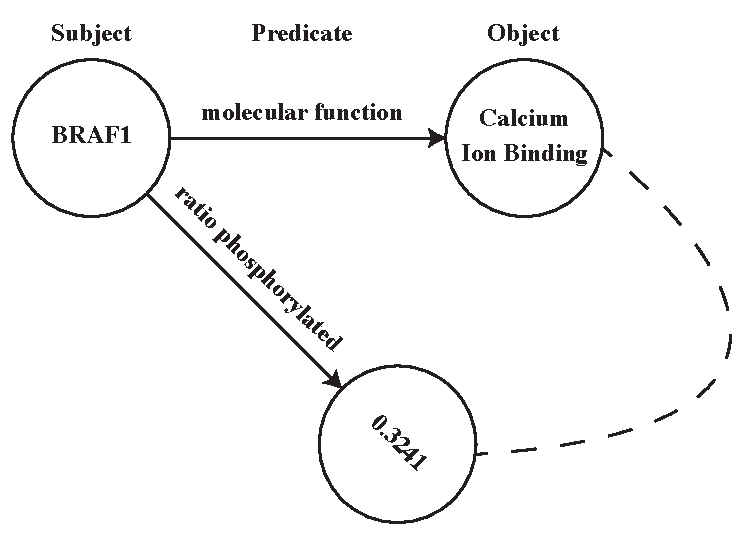
\includegraphics[width=0.75\textwidth]{rdf.pdf}
    \caption{\textbf{General outline of RDF.} Two triples (as shown in \textbf{A}) can be linked by their common subjects (as shown in \textbf{B}), one can infer the relationship between the two objects via the predicates and find patterns: a gene, responsible for calcium ion binding, has a low phosphorylation level in the investigated sample.}
    \label{fig:rdf}
\end{figure}
\noindent
When data is incorporated in a Semantic Web RDF-database (TripleStore) and a relevant set of subjects, predicates and objects are extracted using SPARQL, the remaining dataset is still enormous. The abstract and complex nature of this "hairball" makes it hard to formalise an analytical problem to solve. \textbf{To create interactive and dynamic visual representations of a dataset, we propose to use of the multidisciplinary theories and methods of \textit{visual analytics}}. \citet{Thomas2005} describe this field in 2005 as "\textit{the science of analytical reasoning facilitated by interactive visual interfaces.}". It uses analytical and statistical methods from fields as computer science and statistics and visualisation-techniques from cognitive and design sciences. Visual analytics enables efficient exploratory analysis of the data by the user. Drug discovery is one of the leading areas in biological visual analytics, as it provides a more cost-effective method for analysing data of clinical trails\cite{Cao2008}.

The JavaScript library "Data-Driven Documents" (\textit{D3.js}) is focussed on structuring data for dynamic web-based visualisation, which makes it well-suited for implementing linked data within visual analytics\cite{Bostock2011}. Moreover, since it is embedded in HTML, additional operators (e.g. buttons, SPARQL-forms) can be added (fig. \ref{fig:nya}). Due to these benefits, the use of D3.js in visual analytics is increasing: a notable biology-specific example of this is Epiviz2\cite{Chelaru2014}. However, this tool only takes an explicit set of data-formats and -levels and -more importantly- only shows a particular genomic region, instead of the complete scope. This can easily lead to cherry-picking, instead of data-focussed formulation and analysis of hypotheses.
\medskip
\begin{figure}[H]
    \centering
    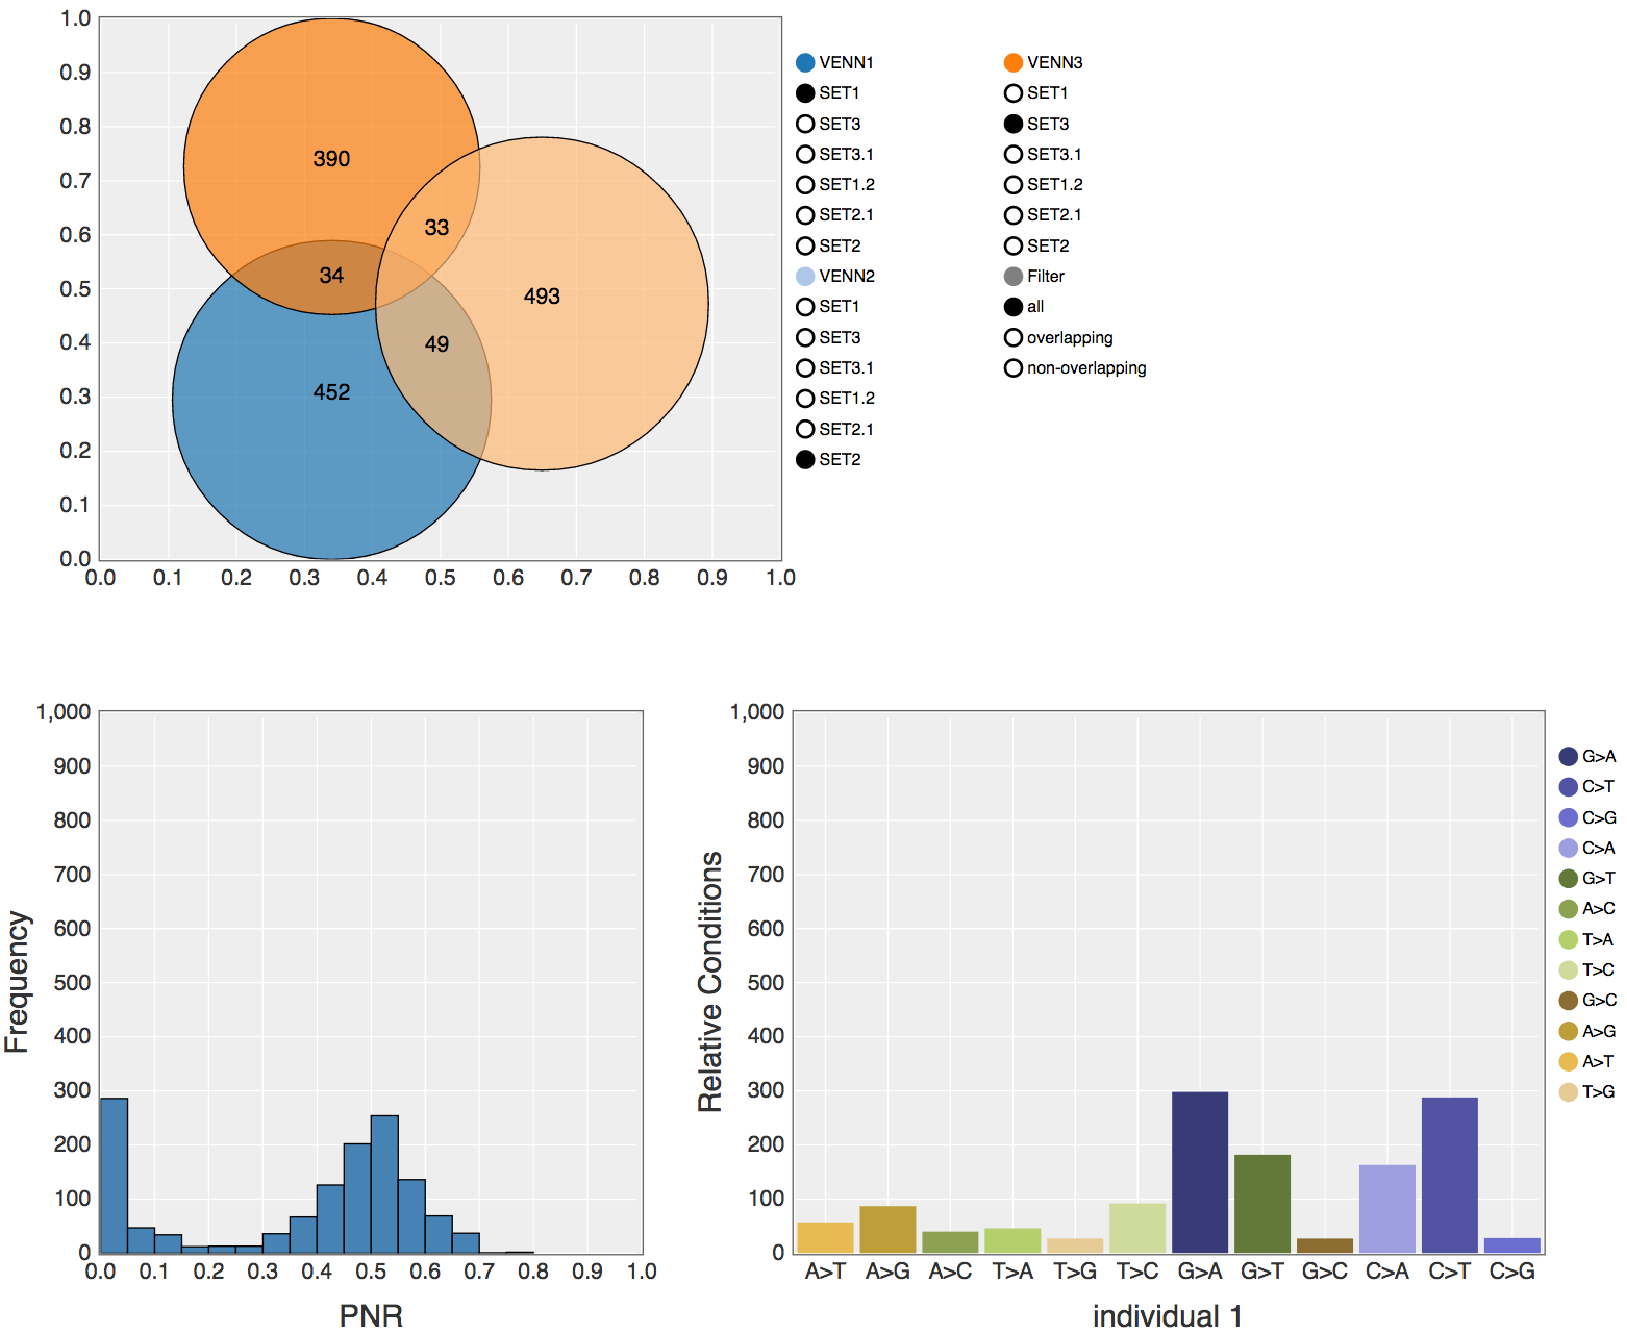
\includegraphics[width=0.75\textwidth]{nyeplot.pdf}
    \caption{\textbf{Visual analytics in d3.js of mutli-sample variants calls} This example shows the possibilities of d3.js and visual analytics: fast and efficient system-wide exploratory analysis of multiple datasets, including cross-talk between the different modules. An interactive version can be found on \url{www.domitry.com/gsoc/multi_pane2.html}.}
    \label{fig:nya}
\end{figure}
\noindent 
The heterogeneous samples and datasets of cancer make it one of the most computationally demanding types of integrative biology. \textbf{We propose to use our methods to study to consequences of structural variations at non-coding loci in cancer on other levels.}  These methods will enable research in this technical challenging topic, by decreasing the computational burden of data-handling, and increase the cognitive abilities of the user, by providing integrative visual interfaces. 
\newpage\subsection*{Originality and innovative character} 
The 2014 survey of \citet{Gomez-Cabrero2014} showed that biomedical academics had the highest interest (78.2 percent) in the integration of multiple omics-datasets and that there was a high need for standardized tools and data-types. Data-storage, -exploration and -exploitation were found the be key. Their conclusions were best summarized by \textit{the need for having exploration tools, which combine summary statistics and interactive visualisations, to analyse heterogeneous data-sets}.
\medskip

\noindent
There have been various studies on the integration of biological signals with the aid of semantic web technologies as the power of ontology-based entailment\footnote{The logical consequence of having two linked ontologies, thereby inferring an additional, encompassing relationship on the shared object/subject} reasoning is widely acknowledged\cite{Sahoo2008}. However, the momentum was lacking: until 2014, big databases were not available in RDF-format. This meant that bioinformatical research involving RDF had little to no outside support, as they could only integrate proprietary data, like the RDF-methods used in microarray analyses by \citet{Szpakowski2009} in 2009. Recently, EMBL-EBI has opened their RDF-platform, boasting six big data-sources (Gene Expression Atlas, ChEMBL, BioModels, Reactome, BioSamples and UniProt)\cite{Jupp2014}. This was the boost needed to further incorporate RDF in biological analyses.

However, there are two main limitations of this relatively young incorporation: a standard language for denoting biological triples (e.g. chromosome locations) is missing and the focus lies at linking database-accessions \citep{Ruttenberg2007}. While the first limitation could also be a strength, as everybody can use their own dialect. However, a standardisation-step will lower the learning-curve, which will enable researchers in all fields of biology to benefit fully from the integrative benefits of the Semantic Web. The second limitation is severely restricting the use of RDF in NGS- and MS-based methods: there are no tools to convert the common formats to triples, like the \textit{Variant Call Format} (VCF) and \textit{Sequence Alignment Format} (SAM). An example of this is  \textit{Bio2RDF}\cite{Belleau2008}: an "\textit{RDFizer}", which converts conventional databases, like the ones from NCBI, to triplestores. One of the leading innovative points of this proposal is the development of methods to handle the NGS- and MS-based formats for use in the Semantic Web. This will result in a broader use of semantic web-technologies for the research community, by enabling the coupling of proprietary NGS- and MS-data to existing RDF-databases.
\medskip

\noindent
%added value of linked data visual analytics TOV standaard methodes ( verwijs naar pilot study)
The implementation of web-based visual analytics for RDF-databases is another leading innovative point in this proposal. Combining Semantic Web-technology with this will create a paradigm shift in the way integrative analysis of (biological) data is done. Visual analytics has been shown to result in the most optimal analysis-effectivity as it allows the user to combine the data with their own background and intuition (fig. \ref{fig:ae}). Not only can data be more effectively analysed, but it can also be better understood and presented, due to the ability to provide an overview of the complete dataset\cite{Thomas2005, Keim}. 
\medskip

\noindent
While there has already been a considerable amount of work in the field of computational cancer research, the vast majority of large-scale integrative studies have been conducted on the coding-regions of the genome\cite{ENCODE}. Genome-Wide Association Studies (GWASs) on a broad range of (hereditary) cancer-types have shown that non-coding locations are associated with these diseases. Until 2013, however, tools and sources to find the precise causative variations in non-coding genomic regions were limited. In the last two years, several advances have made it possible to assess the consequences of individual variations in non-coding regions\cite{Ongen2014,Khurana2013}. However, no large-scale integrative studies have been performed, which is partly due to the current state of integrative methods. 

Due to the affiliation with the University Medical Center Utrecht (UMCU), we are in a unique position to test our hypotheses and methods in both research and clinical settings. Furthermore, the HUB-biobank in the Hubrecht Institute also enables us to perform analyses on organoids, providing us a stable and homogeneous \textit{in vitro} platform for (validation-)studies on cancer-samples. With the new methods, we will be in a position to perform fully integrative studies on the underlying mechanisms and consequences of (structural) variation in cancer.
\medskip
\begin{figure}[h!]
    \centering
    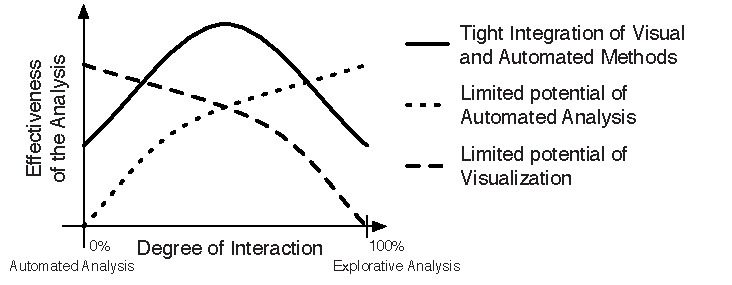
\includegraphics[width=0.75\textwidth]{autoVSexplo.pdf}
    \caption{\textbf{Trade-offs between automated and explorative analysis.} By combining automated analyses, where appropriate, with the background and intuition of the user, an optimal amount of effectivity can be attained. Picture taken from \citet{Keim}.}
    \label{fig:ae}
\end{figure}

\subsection*{Methods and techniques} %M&M
%=================================================
%=================================================
%Describe the overall strategy, methodology, and analyses to be used to accomplish the specific aims of the project. Include how the data will be collected, analyzed, and interpreted as well as any resource sharing plans as appropriate.
%Discuss potential problems, alternative strategies, and benchmarks for success anticipated to achieve the aims.
%As applicable, also include the following information as part of the Research Strategy, keeping within the three sections listed above: Significance, Innovation, and Approach.
%=================================================
%=================================================
Data acquisition will be performed throughout the study. Ongoing sequencing efforts from the research group of Prof. Dr. Cuppen and collaborators will ensure more than adequate amounts of data will be at our disposal. Due to the accompanied scientific questions of this data, the method-development stages of this study will continue to be focussed and inspired by the end-goal: answering biological questions. Furthermore, continuing the data-acquisition in the second half of the study to will enable us to collaborate with the research community and showcase our innovative technology with new and exciting integrative biology studies.
\medskip

\noindent
To ensure the greatest compatibility and effectiveness, tight collaborations will be established between leading RDF-users and -developers in- and outside of biology. Triples for NGS- and MS-based data will be developed, taking into account the most commonly used format first. Since different databases can require a specific triple-structure, RDF-databases will be investigated on their ability to handle the large datasets efficiently, including their in- and output options. Selected research groups in Utrecht will be attracted to provide early feedback-rounds, focussed on usability and compatibility. 

After completion of the triple-development of a data-format (i.e. end-users and the RDF-community have provided positive feedback), development of the conversion-tools is next. In this stage, we seek to expand the capabilities of current leading bioinformatical tools like Sambamba\cite{Tarasov2014} and BIO-VCF\cite{Goto2010}, to capitalise on their multi-core capabilities. Furthermore, we will seek to collaborate with the current (public data-focussed) initiatives, like Bio2RDF\cite{Belleau2008} and BioInterchange\cite{Baran} to ensure software-compatibility and limit redundancy.
\medskip

\noindent
The visualisation-subproject will have two phases. In the first phase, we will use a minimalistic model to develop the link between the SPARQL in- and output and \textit{d3.js}-visualisation. The minimalistic model comprises of SNP- and RNA-based visual analytics-based solutions. Resulting methods can be directly used in other projects, focussing on the role of SNPs and transcription(-levels).

After a successful first phase, the second phase will broaden the available visualisations, by creating a modular dashboard. Every module will provide a particular visual (e.g. heat-map, scatter-plot) and will interact with both the SPARQL-input, -output and the other active modules. If a user would, for example, select a specific gene in the scatter-plot, the same data-point will be highlighted in the other modules. The cross-talk between modules has already been implemented in Epiviz2\cite{Chelaru2014}, which is highly appraised for this by its users. The order of development of specific modules will be primarily based on the wants and needs of the community, which will be gathered with the above-mentioned feedback-rounds.
%\newpage
\subsection*{Pilot-study}
To asses to feasibility of this proposal, a small-scale pilot-study was performed on de data of \citet{VanHeesch2014}. This dataset includes transcriptome data of mRNA's, bound to a number of ribosomal units (1 to 7+) and matching exome-data. If one would be interested in the molecular functions of a gene with an allelic bias, a disproportional amount of time is lost on parsing, intersecting and downloading various types of data (fig. \ref{fig:awesome_image}). With the current methods, twelve set-operations (e.g. intersections, unions) have to be performed on $\pm$5gb of data. Furthermore, three datasets ($\pm$15gb) have to be completely downloaded once -until a new version is launched- before a simple exploratory question can be answered. Approximately three and a half hours was needed to perform this, in contrast to one hour with the proposed methods. Of this hour, more than fifty minutes were used to convert VCF to RDF and load the 4store database: every query hereafter takes up approximately 10 minutes. First and foremost, this pilot illustrates the low-complex nature of the proposed methods. Secondly, it shows the valuable property of having a separate query-stage, which results in being able to make more than ($\frac{(8*60)-50}{10}= $) forty queries in eight hours, instead of approximately ($\frac{8-3,5}{3,5}= $) two queries with the currently used methods.
\begin{figure}[h!]
    \centering
    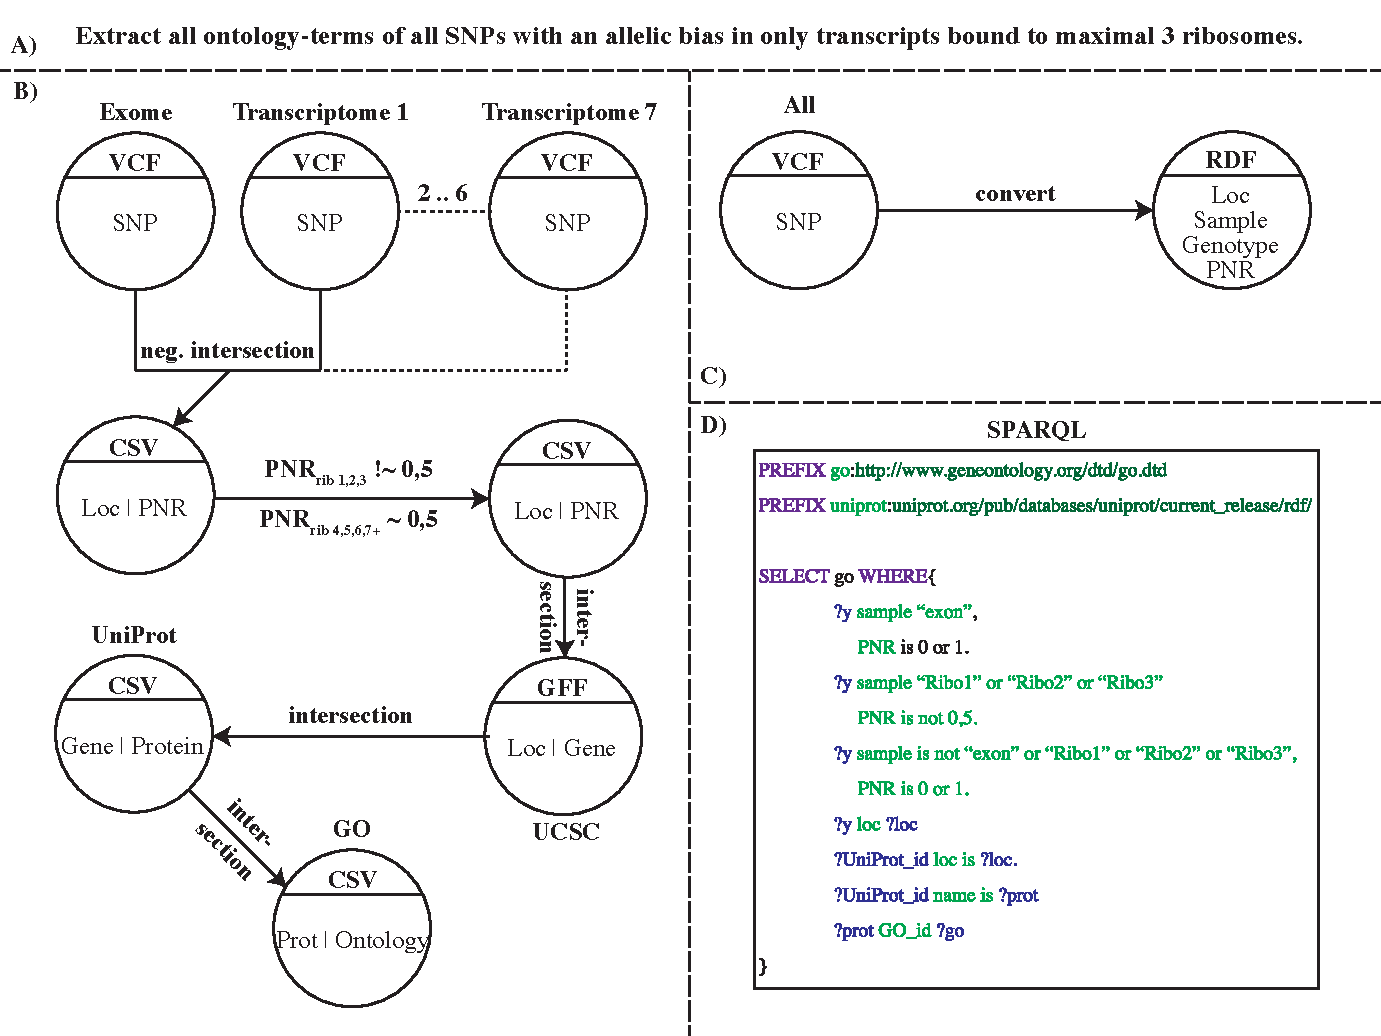
\includegraphics[width=0.75\textwidth]{DifferencesInDoingThings}
    \caption{\textbf{Differences between current integration techniques and RDF.} When a researcher has a question like \textbf{A}, they have to go through a series of parsing and interception steps, like in \textbf{B}. External sources have to be fully downloaded and converted, before use. Our proposed pipeline (shown in \textbf{C}), firstly converts the data to RDF. Then, a question can be formulated in SPARQL (\textbf{D}), incorporating relevant outside sources, which can be easily changed without having to juggle/download the data again.}
    \label{fig:awesome_image}
\end{figure}
\newpage
\section*{Research plan}
\subsection*{Timetable}
\begin{table}[h]
\begin{center}
\begin{tabular}{lllllll}
                                                & \multicolumn{6}{c}{Semesters}                                                                                                                                                                                                                                                                                                                                                                                 \\ \cline{2-7} 
                                                & S1                                              & S2                                              & S3                                              & S4                                              & S5                                              & S6                                                                                          \\ \hline
\textbf{Data acquisition}               &           & \cellcolor[HTML]{343434}{\color[HTML]{656565} } & \cellcolor[HTML]{343434}{\color[HTML]{656565} } & \cellcolor[HTML]{343434}{\color[HTML]{656565} } & \cellcolor[HTML]{343434}{\color[HTML]{656565} } & \cellcolor[HTML]{343434}{\color[HTML]{656565} }   \\
\textbf{Aim 1: Data-integration}                & \cellcolor[HTML]{343434}                        & \cellcolor[HTML]{343434}                                             &                                                 &                                                 &                                                                                              \\
\hspace*{1em} Developing omics-specific triples & \cellcolor[HTML]{656565}                        &                                                 &                                                 &                                                 &                                                 &                                                                                                 \\
\hspace*{1em} Coding conversion-tools           &                                                 \cellcolor[HTML]{656565}               &     \cellcolor[HTML]{656565}         &                      &                                                 &                                                 &                                                                                                \\
\hspace*{1em} Writing Best-Practices            &                                                 &                                                  \cellcolor[HTML]{656565}             &           &                                                 &                                                                                                  &                                                                                                \\
\textbf{Aim 2: Visual analytics}                &                                                 &                                                  \cellcolor[HTML]{343434}                        & \cellcolor[HTML]{343434}                        &                                                                                                                        &                                                 \\
\hspace*{1em} Coding SPARQL+D3 endpoint         &                                                 &                                                  \cellcolor[HTML]{656565}                        &                                                 &                                                                                                 &                                                 &                                                 \\
\hspace*{1em} Adding visualisation-methods      &                                                                                               & \cellcolor[HTML]{656565}                        & \cellcolor[HTML]{656565}                                                                         &                                                 &                                                 &                                                 \\
\hspace*{1em} Adding filtering and output                                                                                           &                                                 &  &                                                \cellcolor[HTML]{656565}   &                                                 &                                                 &                                                 \\
\textbf{Aim 3: Multi-level analysis}            &                                                                                                  &                                                 &  & \cellcolor[HTML]{343434}{\color[HTML]{343434} } & \cellcolor[HTML]{343434}{\color[HTML]{343434} } & \cellcolor[HTML]{343434}{\color[HTML]{343434} } \\
\hspace*{1em} Non-coding structural factors of drug-resistance                                                        &                                                 &                                                 &                        & \cellcolor[HTML]{656565}                  & \cellcolor[HTML]{656565}                     &                    \\
\hspace*{1em} Single-cell analysis of SVs in cancer sub-populations                                                       &                                                 &                                                 &                        &                & \cellcolor[HTML]{656565}                     & \cellcolor[HTML]{656565}                   \\

\textbf{Writing thesis}                         &                                                 &                                                 &                                                 &                                                 &                                                                        & \cellcolor[HTML]{343434}                       
\end{tabular}
\end{center}
\end{table}
\subsection*{Proposed biological questions}
Semester four to six will be used to perform multi-level analysis with the resulting methods and tools from the previous three semesters. The overall aim is to combine both proprietary and public data to execute previously impossible analyses. Of the public databases available, the most valuable for our purposes are those, that link omics-data to pathways and ontologies: \textit{Pathway Commons}\cite{Cerami2011} and \textit{Reactome}\cite{Jupp2014} on perturbed pathways in cancer, \textit{RegulomeDB}\cite{Boyle2012} on linking non-coding regions to genes and \textit{Gene Ontology}\cite{Ashburner2000} and \textit{KEGG-pathway}\cite{Kanehisa2000} for general ontologies and pathways. A subset of the addressed questions and proposed analyses is depicted below.
\renewcommand{\labelenumi}{\roman{enumi}.}
\begin{enumerate}
\item \textbf{Non-coding structural factors of drug-resistance} \\
The Cancer Genomics Centre Netherlands (CGC.nl) is in the process of studying the effects of variants in coding regions in cancer, including factors of drug resistance. However, the data has not been used to study the non-coding regions, primarily because of the aforementioned limitations in both non-coding analysis and data-integration. Firstly, we will analyse the (epi)genomic data to identify cancer-specific SVs that are cis-acting on specific genes. Secondly, the data of the products of these genes (e.g. transcripts, proteins and metabolites) is integrated to infer possible consequences on these levels. Linking specific drug-resistance information will also enable us find patterns between the SVs, the identified (consequences of) genes and specific drugs. Since treatment of a single drug often leads to resistance by a bypass in the drug-inhibited pathway\cite{Prahallad2012}, we also integrate public and CGC.nl-data on perturbed pathways in cancer. This will elucidate the mechanisms of non-coding SV-induced drug-resistance in cancer samples and potentially identify new targets for treatment.
\item \textbf{Single-cell analysis of SVs in cancer sub-populations} \\
Due to the advances in single-cell sequencing (CELL-seq) of both DNA and RNA, we are able to look at consequences of SVs on transcription in single cells. The innovation here is the fact that signals are not averaged out by multiple (asynchronous) cells and we can thus analyse the cell as part of a sub-population. By integrating CELL-seq DNA- and RNA-data of different sub-populations of (heterogeneous) cancer-samples, we can find the previously obscured direct (i.e. cis-acting) and indirect (i.e. trans-acting) consequences of SVs in specific sub-populations. Furthermore, integrating data of lineage-tracing between and within different sub-populations could identify causal non-coding SV-events in the progression of cancer. Linking the public data of ontology- and pathway-databases will enable us to infer specific sub-population changes in pathways as the consequence of SVs or de-regulated genes due to SVs.
\end{enumerate}
This subset of questions shows the main innovative point of our proposed methods: they make it possible to efficiently and systematic analyse and integrate several omics-levels and multiple dimensions (e.g. drug-resistance, cancer type/sub-population), while allowing easy connection to public data.



\subsection*{Collaboration}
By performing this research in the Hubrecht Institute, we surround ourself with various research-fields within the scope of Developmental Biology. One of the newest findings of the Hubrecht are Organoids, which provide a method to study heterogeneous tissues (e.g. cancer) in more detail, by providing clonal (i.e. homogeneous) cultured tissues. Groups in the Hubrecht are heavily involved in (inter)national consortia, like the \textit{Cancer Genomics Centre}. This national consortium of research-groups, predominantly of the Hubrecht Institute and the Netherlands Cancer Institute (NKI), focusses on cancer's (epi)genetic alterations and responses to drugs. Data from this project will include various levels (e.g. (epi)genomics, phosphomics) and dimensions (e.g. drug-responses, time-series). For the cancer sub-population study, a collaboration between the \textit{van Oudenaarden}-group (lineage-tracing and CELL-seq) and the \textit{Clevers}-group (cancer-biobank) will be formed.

Furthermore, the affiliation between the institute and Utrecht University will lead the more possibilities. A considerable amount research groups make use of the Utrecht DNA-sequencing Facility and the Netherlands Proteomics Centre, which ensures adequate amounts and variation in data and data-integration-based research questions. 

Ties with international leaders in biology-related semantic web and visualisation technologies have been made and will continue to be expanded. Joachim Baran and Pjotr Prins have been heavily involved in the planning stages, being key players in handling various data-formats (into RDF) with \textit{BIO-Ruby}. Communications with Artem Tarasov of \textit{Sambamba} and Jerven Bolleman -key engineer of the \textit{UniProt-RDF} project- have also been established.
\section*{Knowledge utilisation}
The implementation of RDF will be swift since RDF already is a web-standard and a significant number of public biology-related sources are already in RDF-format. This will enable users of our methodologies to efficiently connect and integrate their data with public resources. Current statistical software, like the R environment, have packages (made by researchers from computer sciences) to extract and further analyse SPARQL-output. This means that users only have to learn SPARQL-queries, in order to use the proposed methods.

By enabling more users to use methods and sources of RDF, this research will, in a broader perspective, have a direct effect on the Semantic Web. By lowering the (bioinformatical) threshold for analysis, more data can be faster analysed by more people, further accelerating research. Users will also be able to tell their story (i.e. results) better. Psychologist will, for example, be able to get a better visualisation and thus understanding of a neuroscientist's work. Big pharmaceutical companies will be able to further include and analyse data of basic science, clinical trails and business-statistics with more efficiency. Moreover, the research-community will be one significant step further in dissecting the complex biology of cancer.


%
%linked data visual analystic zijn in alle velden te grebruiken, die RDf gebruiken. Ook voor bedrijven (pharma!). Super handig!
%
%Vrij snel te incorpporeren: de meeste dingen zijn er al
%
%cancer NC-SV is nog weinig over bekend: mogelijke nieuwe targets voor cancer screening and or treatment: sociaal en pharma.




%-------------------------------------------------------
%	REFERENCE LIST
%----------------------------------------------------------------------------------------

%\begin{thebibliography}{99} % Bibliography - this is intentionally simple in this template

%\renewcommand{\refname}{\LARGE\scshape\centering References} %
%\titleformat*{\section}{\LARGE\scshape\centering}
%\titleformat{\section}[block]{\LARGE\scshape\centering}{\thesection.}{1em}{} % Change the look of the section titles
\begin{tiny}

\bibliography{library}
 \end{tiny}
%\end{thebibliography}
%
%%----------------------------------------------------------------------------------------
%
%%\end{multicols}

\end{document}
